\documentclass[twoside]{article}
\input{ISC18-english.sty}
%%%%%%%%%%%%%%%%%%%%%%%%%%%%  Make sure to compile twice for proper cross-references. %%%%%%%%%%%%%%%%%%%%%%%
%%%%%%% For proper display of references, compile the document twice. %%%%%%%%%%%%%%%%%%%%% 
%%%%%%%%%%%%%%% If using TeX Live, compile using pdflatex command %%%%%%%%%%%%%%%%%%%%%%%
\begin{document}
\thispagestyle{empty}
%%%%%%%%%%%%%%%%% Article title header  %%%%%%%%%%%%%%%%%%%%
\fancyhead[LE]{Estimation of Reliability for Gompertz Distribution Under RSS}
%%%%%%%%%%%%%%%%% Article authors header   %%%%%%%%%%%%%%%%%%%%
%\fancyhead[RO]{Z. Karimiezmareh}
\begin{center}
{
\includegraphics [height=25mm, width=150.3mm] {Images/isc18E}} \\
\vspace*{-1.8cm}
%\begin{center}
%\color{blue} 
%{\hspace{0.1cm}\rule{\textwidth}{1mm}}\\
%\end{center}
\vspace*{4cm}
%%%%%%%%%%%%%%%%% Article title  %%%%%%%%%%%%%%%%%%%%
{\Large \bf Efficient Bayesian Inference for Stress-Strength Reliability in Gompertz Distribution via Ranked Set Sampling}\\
%%%%%%%%%%%%%%%%% Article authors and affiliations %%%%%%%%%%%%%%%%%%%%
%{\bf
%Zahra Karimiezmareh  \footnote[1]{{\bf Corresponding Author:} {\tt zahra.karimiez@atu.ac.ir }} \\
%$^1$Department of Statistics, Allameh Tabataba’i University, Tehran, Iran \\
%%$^2$Second Author's Affiliation
%}
\end{center}
\rule{\textwidth}{0.2mm}\\
%%%%%%%%%%%%%%%%% Article abstract  %%%%%%%%%%%%%%%%%%%%
\noindent{\bf Abstract:}\\
The Gompertz distribution, with its exponentially increasing hazard rate, is widely used in reliability engineering and survival analysis. However, estimating stress-strength reliability under this distribution has received limited attention. Conventional simple random sampling (SRS) is inefficient when precise measurements are costly or time-consuming. Ranked set sampling (RSS) addresses this limitation by using inexpensive ranking before measurement, extracting more information without increasing sample size. This study develops a Bayesian estimation of stress-strength reliability 
$R=P(X<Y)$ for the Gompertz distribution under RSS. Bayesian estimators are derived under a squared error loss function using the Metropolis-Hastings algorithm. The significance of this work is providing an efficient, low-cost, and high-precision method for reliability estimation when accurate measurement is expensive or difficult.
 
\noindent{\bf Keywords:} 
Ranked Set Sampling, Gompertz Distribution, Stress-Strength Reliability, and Metropolics-Hastings Algorithm. \\
\noindent{\bf Mathematics Subject Classification (2020):} $\rm 62Exx$, $\rm 62F10$, $62F15$. \\
\hspace{1cm}\rule{\textwidth}{0.2mm}\\
%%%%%%%%%%%%%% 
\section{Introduction}

\cite{gompertz1825xxiv} discovered that after adulthood, the risk of death increases exponentially with age and applied this law to help insurance companies that needed reliable mortality tables but had limited, outdated data. Instead of relying solely on raw data, he proposed fitting a smooth exponential curve to mortality figures. This approach filled data gaps and enabled reasonable predictions of death rates for very old ages.
 %Thus, Gompertz’s law provided a practical, data-driven method for improving actuarial calculations.
%\cite{gompertz1825xxiv} found that the risk of death for humans after reaching adulthood increases exponentially with age. Using this mathematical law, Gompertz provided a practical solution to an important business problem. Insurance companies needed "mortality tables" to calculate life insurance premiums. These tables were based on limited and outdated data and were unreliable for predicting the risk of death at different ages, especially for older ages where data were scarce. Gompertz suggested that instead of relying solely on the raw mortality table data, one could fit a smooth, continuous curve to mortality data using his exponential law. This had two major advantages: it allowed for gaps in the data at ages where there was insufficient information, and it made it possible to reasonably predict mortality rates for very old ages.
The Gompertz distribution models time-to-event data with an exponentially increasing hazard rate and has been generalized to improve flexibility. In medicine, the Generalized Exponentiated Unit Gompertz Distribution by \cite{sindhu2024generalized} successfully modeled arthritic pain relief times. Additionally, the Exponentiated Generalized Exponential Gompertz Distribution by \cite{ezmareh2025exponentiated} further advances reliability and survival analysis. The practical use of these models relies on robust statistical inference for complex data structures. This need is addressed by \cite{lv2024statistical}, who developed inference methods for general progressive Type II censored competing risks samples. %These developments highlight the ongoing evolution of the Gompertz family. The extended models provide improved fit for real-world datasets. Their utility depends on effective handling of censored and competing risks data. Overall, these advancements expand the applicability of Gompertz distributions across various fields.




\begin{dfn}\label{df1}
A continuous random variable $X$ on the interval $[0,\infty)$ has a Gompertz distribution with parameters $\beta>0$ and $\gamma>0$, denoted by $G(\beta, \gamma)$, if its probability density function (PDF) and cumulative distribution function (CDF) are respectively:
\begin{align}\label{1}
& f(x)=\beta e^{\gamma x}e^{-\frac{\beta}{\gamma}(e^{\gamma x}-1)},\\ \label{2}
& F(x)=1-e^{-\frac{\beta}{\gamma}(e^{\gamma x}-1)}.
\end{align}
\end{dfn}


The stress-strength reliability $R = P(\text{Strength} > \text{Stress})$ is a critical metric for assessing safety margins and failure risks in engineering design. \cite{hakamipour2025stress} enhanced multicomponent system analysis by modeling dependent component strengths using copula functions. \cite{hudaverdi2023copula} addressed scenarios with two correlated stress sources via a bivariate copula-based framework. \cite{karimi2022statistical} derived inference procedures for stress-strength reliability under the Gompertz distribution with Type II censoring. These advances enable more realistic reliability assessment under complex dependencies. %Overall, recent research has significantly improved stress-strength modeling for practical engineering applications.

Ranked Set Sampling (RSS), introduced by \cite{mcintyre1952method}, is an efficient technique when measurement is costly but ranking is cheap. It involves visually ranking small random subsets and then precisely measuring only the top-ranked unit from each subset. This structured approach minimizes sampling variability and provides more informative data. As a result, RSS yields significantly more precise parameter estimates than Simple Random Sampling (SRS) with the same measurement effort.

To construct an RSS sample of size $n$, draw $m$ independent sets of size $m$ via SRS, rank units within each set without precise measurement, and select the $r$-th ranked unit from the $r$-th set. This yields one cycle of RSS with observations $X_{(1)1},\ldots,X_{(m)m}$. Repeating the procedure across $k$ independent cycles gives a total sample of size $n=mk$, denoted as $X_{(1)1c},\ldots,X_{(m)mc}$ for $c=1,\ldots,k$. For convenience, we write $X_{rc}$ in place of $X_{(r)rc}$. %These observations are mutually independent but, in general, not identically distributed.
%To construct a sample of size $n$ using the RSS approach, draw $m$ independent sets, each of size $m$, from the population through SRS. The elements within each set are then ordered according to some auxiliary criterion without performing exact measurements. From the $r$-th set, the unit ranked in the $r$-th position is chosen for precise measurement, where $r = 1,2,\ldots,m$. The resulting collection of measured observations, denoted by $X_{(1)1},\ldots,X_{(m)m}$, is defined as one cycle of RSS. Repeating this procedure across $k$ independent cycles yields a total sample size of $n=mk$. The combined data set can be written as $X_{(1)1c},\ldots,X_{(m)mc}$, for $c=1,\ldots,k$. For notational convenience, we use $X_{rc}$ in place of $X_{(r)rc}$. These observations are mutually independent but, in general, not identically distributed. The PDF and CDF of $X_{rc}$ are given by
\begin{align}
&f_{r:m}(x)=\frac{m!}{(r-1)!(m-r)!}[F(x)]^{r-1}[1-F(x)]^{m-r}f(x),\\
&F_{r:m}(x)=\sum_{i=r}^{m}\binom{m}{i}[F(x)]^{i}[1-F(x)]^{m-i}.
\end{align}
Estimating stress-strength reliability using RSS represents a significant advancement in reliability engineering, as RSS's structured data collection mechanism systematically captures greater information from the population compared to SRS. \cite{basikhasteh2020bayesian} successfully addressed the complexities of estimating $R$ for a bathtub-shaped lifetime distribution by developing a Bayesian framework within a maximum RSS design. \cite{aldrabseh2025enhanced} established that even for the classical exponential distribution, sophisticated RSS variants yield substantial improvement in estimation accuracy.

Accurate estimation of stress-strength reliability in Gompertz models remains challenging due to the statistical limitations of conventional sampling methods. Traditional reliability assessments using SRS often fail to achieve statistical efficiency, particularly when dealing with exponentially-increasing hazard rates and resource-intensive measurements. Our research addresses this limitation by integrating RSS within a Bayesian paradigm. 
%Accurate estimation of stress-strength reliability in Gompertz models is challenging due to limitations of conventional sampling methods, especially with exponentially-increasing hazard rates and costly measurements. Our research addresses this by integrating RSS within a Bayesian paradigm to improve statistical efficiency.

\section{Bayesian Estimation of Parameters}\label{sec2}
In this section, Bayesian estimation of the Gompertz distribution parameters is obtained based on SRS and RSS. A Gamma prior distribution is used, and estimates are obtained under the squared error (SEL) loss function.

\subsection{Estimation Based on SRS}

Assume $\beta$ has a Gamma prior with parameters $(a_1, b_1)$, and $\gamma$ has a Gamma prior with parameters $(a_2, b_2)$. The joint posterior density is proportional to the product of the likelihood and prior:
\begin{equation}
\pi(\beta,\gamma\mid X)\propto\beta^{n+a_1-1}e^{-b_1\beta}\gamma^{a_2-1}e^{-b_2\gamma}e^{\gamma\sum x_i}e^{-\frac{\beta}{\gamma}\sum(e^{\gamma x_i}-1)}.
\end{equation}

The conditional posterior densities are:
\begin{align}
&(\beta\mid\mathbf{x},\gamma)\sim\text{Gamma}\left(n+a_1,\;b_1+\frac{1}{\gamma}\sum_{i=1}^n(e^{\gamma x_i}-1)\right),\\
&\pi(\gamma\mid\mathbf{x})\propto\gamma^{a_2-1}e^{-\gamma(b_2-\sum x_i)}e^{-\frac{\beta}{\gamma}\sum(e^{\gamma x_i}-1)}.
\end{align}
Although samples for $\beta$ are straightforward to draw, generating samples for $\gamma$ requires the Metropolis-Hastings algorithm.

\subsection{Estimation Based on RSS}

Suppose we have an RSS of size $n=mk$, denoted by $X_{ic}$ for $i=1,\ldots,m$ and $c=1,\ldots,k$, which follows $G(\beta,\gamma)$. Based on Equations \eqref{1} and \eqref{2}, the PDF of $X_{ic}$ is:
\begin{align}
g(x_{ic}\mid\beta,\gamma)=
%\sum_{r=0}^{i-1}i\binom{m}{i}\binom{i-1}{r}(-1)^r f(x_{ic}\mid\beta,\gamma)[1-F(x_{ic}\mid\beta,\gamma)]^{m+r-i}\nonumber\\
\sum_{r=0}^{i-1}i\binom{m}{i}\binom{i-1}{r}(-1)^r\beta e^{\gamma x_{ic}}e^{-\frac{\beta}{\gamma}(e^{\gamma x_{ic}}-1)(m+r-i+1)}.
\end{align}
Considering $\mathbf{x}=(x_{1c},\ldots,x_{mc})$, the joint density is:
\begin{align}\label{Post}
g(\mathbf{x}\mid\beta,\gamma)&=\prod_{c=1}^k\prod_{j=1}^m g(x_{jc}\mid\beta,\gamma)\notag\\
&=\prod_{c=1}^k\Biggl\{\sum_{i_1=0}^0\sum_{i_2=0}^1\cdots\sum_{i_m=0}^{m-1}\Biggl[\prod_{j=1}^m j\binom{m}{j}\binom{j-1}{i_j}(-1)^{i_j}\Biggr]\notag\\
&\quad\times\beta^m e^{\gamma\sum_{j=1}^m x_{jc}}e^{-\frac{\beta}{\gamma}\sum_{j=1}^m(m+i_j-j+1)(e^{\gamma x_{jc}}-1)}\Biggr\}.
\end{align}
From Equations \eqref{Post} and the joint prior distribution, the joint posterior distribution for RSS is:
\begin{align}
\pi(\beta,\gamma\mid\mathbf{x})&\varpropto\prod_{c=1}^k\Biggl\{\sum_{i_1=0}^0\cdots\sum_{i_m=0}^{m-1}\prod_{j=1}^m j\binom{m}{j}\binom{j-1}{i_j}(-1)^{i_j}\notag\\
&\quad\times\beta^{m+a_1-1}e^{-b_1\beta}\gamma^{a_2-1}e^{-\gamma[b_2-\sum_{j=1}^m x_{jc}]}e^{-\frac{\beta}{\gamma}\sum_{j=1}^m(e^{\gamma x_{jc}}-1)(m+i_j-j+1)}\Biggr\}.
\end{align}
This equation does not have a known distribution form, so we use MCMC to sample from it. Note that:
\begin{align}
\pi(\beta\mid\mathbf{x},\gamma)&\varpropto\prod_{c=1}^k\Biggl\{\sum_{i_1=0}^0\cdots\sum_{i_m=0}^{m-1}\prod_{j=1}^m j\binom{m}{j}\binom{j-1}{i_j}(-1)^{i_j}\notag\\
&\quad\times\beta^{m+a_1-1}e^{-\beta[b_1+\frac{1}{\gamma}\sum_{j=1}^m(e^{\gamma x_{jc}}-1)(m+i_j-j+1)]}\Biggr\},\\
\pi(\gamma\mid\mathbf{x},\beta)&\varpropto\prod_{c=1}^k\Biggl\{\sum_{i_1=0}^0\cdots\sum_{i_m=0}^{m-1}\prod_{j=1}^m j\binom{m}{j}\binom{j-1}{i_j}(-1)^{i_j}\notag\\
&\quad\times\gamma^{a_2-1}e^{-\gamma[b_2-\sum_{j=1}^m x_{jc}]}e^{-\frac{\beta}{\gamma}\sum_{j=1}^m(e^{\gamma x_{jc}}-1)(m+i_j-j+1)}\Biggr\}.
\end{align}

\section{Estimation of Stress-Strength Reliability}\label{sec3}

Consider two independent random variables: $X\sim G(\beta_1,\gamma)$ and $Y\sim G(\beta_2,\gamma)$. The stress-strength reliability $R$ is:
\begin{align}
\large R &= \large P (\large X < \large Y)\\
& = \int_{0}^{\infty} F_{X}(y)f_{Y}(y) dy \notag \\
	& = \int_{0}^{\infty} (1-e^{-\frac{\beta_{1}}{\gamma}(e^{\gamma x} -1 )})(\beta_{2}e^{\gamma y}e^{-\frac{\beta_{2}}{\gamma}(e^{\gamma y} -1 )})dy
	 \notag \\
	& = 1-\int_{0}^{\infty} \beta_{2}e^{\gamma y}e^{-\frac{ 1}{\gamma}(e^{\gamma y} -1 )(\beta_{1} +\beta_{2})}dy
	 \notag \\
	& = 1- \frac{\beta_{2}}{\beta_{1} + \beta_{2}} = \frac{\beta_{1}}{\beta_{1} + \beta_{2}}\cdot
\end{align}

\subsection{R Estimation Based on SRS}

Let $\mathbf{X}=(X_1,\ldots,X_n)$ and $\mathbf{Y}=(Y_1,\ldots,Y_m)$ be two independent SRS from $X$ and $Y$. The likelihood function for $\boldsymbol{\theta}=(\beta_1,\beta_2,\gamma)$ is:
\begin{align}
L(\boldsymbol{\theta}\mid\mathbf{x},\mathbf{y})\propto\beta_1^n\beta_2^m e^{\gamma(\sum x_i+\sum y_j)}e^{-\frac{1}{\gamma}[\beta_1(\sum e^{\gamma x_i}-n)+\beta_2(\sum e^{\gamma y_j}-m)]}.
\end{align}
We assume independent priors: $\beta_1\sim\text{Gamma}(a_1,b_1)$, $\beta_2\sim\text{Gamma}(a_2,b_2)$, $\gamma\sim\text{Gamma}(a_3,b_3)$. The joint posterior is:
\begin{align}
\pi(\boldsymbol{\theta}\mid\mathbf{x},\mathbf{y})&\propto\beta_1^n\beta_2^m e^{\gamma(\sum x_i+\sum y_j)}e^{-\frac{1}{\gamma}[\beta_1(\sum e^{\gamma x_i}-n)+\beta_2(\sum e^{\gamma y_j}-m)]}\notag\\
&\quad\times\beta_1^{a_1-1}e^{-b_1\beta_1}\beta_2^{a_2-1}e^{-b_2\beta_2}\gamma^{a_3-1}e^{-b_3\gamma}.
\end{align}
The full conditional distributions are:
\begin{align}
&(\beta_1\mid \beta_2 , \gamma , \mathbf{x},\mathbf{y} )\sim\text{Gamma}\left(n+a_1,\;b_1+\frac{1}{\gamma}\sum_{i=1}^n(e^{\gamma x_i}-1)\right),\\
&(\beta_2\mid \beta_1 , \gamma , \mathbf{x},\mathbf{y} )\sim\text{Gamma}\left(m+a_2,\;b_2+\frac{1}{\gamma}\sum_{j=1}^m(e^{\gamma y_j}-1)\right),\\
&\pi(\gamma\mid \beta_1 , \beta_2 , \gamma , \mathbf{x},\mathbf{y} )\propto\gamma^{a_3-1}e^{\gamma(\sum x_i+\sum y_j-b_3)}e^{-\frac{1}{\gamma}[\beta_1\sum(e^{\gamma x_i}-1)+\beta_2\sum(e^{\gamma y_j}-1)]}.
\end{align}

\subsection{R Estimation Based on RSS}

Let $\mathbf{X}=\{X_{ic}, i=1,\ldots,m_x, c=1,\ldots,k_x\}$ and $\mathbf{Y}=\{Y_{jr}, j=1,\ldots,m_y, r=1,\ldots,k_y\}$ be two independent RSS samples from $\text{Gompertz}(\beta_1,\gamma)$ and $\text{Gompertz}(\beta_2,\gamma)$, respectively. The joint posterior distribution is:
\[
\pi(\boldsymbol{\theta}\mid\mathbf{x},\mathbf{y})\propto g(\mathbf{x}\mid\beta_1,\gamma)\,g(\mathbf{y}\mid\beta_2,\gamma)\,\pi(\beta_1)\pi(\beta_2)\pi(\gamma).
\]

Due to the complexity of the full conditional distributions, we use the Metropolis-Hastings algorithm with proposal $q(\boldsymbol{\theta})\propto q(\beta_1)q(\beta_2)q(\gamma)$, where $q(\beta_1), q(\beta_2), q(\gamma)$ are independent half-normal densities. The sampling procedure:

\noindent\textbf{Step 1:} Initialize $\boldsymbol{\theta}^{(0)}=(\beta_1^{(0)},\beta_2^{(0)},\gamma^{(0)})'$, set $t=1$.

\noindent\textbf{Step 2:} Generate $\beta_1^{(t)}$ from $q(\beta_1)$ and form $\boldsymbol{\theta}^{(t)}=(\beta_1^{(t)},\beta_2^{(t-1)},\gamma^{(t-1)})'$. Accept with probability
\[
\rho=\min\left\{\frac{\pi(\boldsymbol{\theta}^{(t)}\mid\mathbf{x},\mathbf{y})}{\pi(\boldsymbol{\theta}^{(t-1)}\mid\mathbf{x},\mathbf{y})}\cdot\frac{q(\boldsymbol{\theta}^{(t-1)}\mid\boldsymbol{\theta}^{(t)})}{q(\boldsymbol{\theta}^{(t)}\mid\boldsymbol{\theta}^{(t-1)})},1\right\}.
\]

\noindent\textbf{Step 3:} Generate $\beta_2^{(t)}$ from $q(\beta_2)$ and set $\boldsymbol{\theta}^{(t)}=(\beta_1^{(t)},\beta_2^{(t)},\gamma^{(t-1)})'$, then accept using $\rho$.

\noindent\textbf{Step 4:} Generate $\gamma^{(t)}$ from $q(\gamma)$ and set $\boldsymbol{\theta}^{(t)}=(\beta_1^{(t)},\beta_2^{(t)},\gamma^{(t)})'$, then accept using $\rho$.

\noindent\textbf{Step 5:} Compute $R^{(t)}=\beta_1^{(t)}/(\beta_1^{(t)}+\beta_2^{(t)})$.

\noindent\textbf{Step 6:} Increment $t$ and repeat Steps 2-5 $N$ times.

The Bayes estimators under SEL loss is:
\[
\hat{R}_{\text{SEL}}=\frac{1}{N-M}\sum_{t=M+1}^N R^{(t)}.
\]
\section{Simulation Study}\label{sec4}
We conducted Monte Carlo simulations to compare the performance of Bayesian estimators of stress-strength reliability \(R = P(X<Y)\) for the Gompertz distribution under SRS and RSS. The simulation parameters were set as follows: number of Monte Carlo runs \(= 300\), MCMC iterations \(= 6000\) with \(1000\) burn-in, number of cycles \(k_x = k_y = 10\), and non-informative priors with hyperparameters \(0.0001\). Three scenarios for \(R\) were considered: \(R = 0.2\) (\(\beta_1 = 0.25, \beta_2 = 1.0\)), \(R = 0.5\) (\(\beta_1 = 0.5, \beta_2 = 0.5\)), and \(R = 0.8\) (\(\beta_1 = 1.0, \beta_2 = 0.25\)), with \(\gamma = 0.5\) fixed. Different set sizes \((m_x, m_y) = (2,2), (3,3), (4,3), (4,4)\) were examined. The mean squared error (MSE), bias, and \(95\%\) highest posterior density (HPD) credible interval length were computed for each scenario.

Table \ref{tab1} presents the MSEs, biases, and HPD lengths of the Bayesian estimates for \(R\) under squared error loss (SEL). The results reveal that the performance of RSS relative to SRS depends on the symmetry of the stress and strength distributions. When \(R = 0.5\), corresponding to symmetric distributions, RSS substantially outperforms SRS. The relative efficiency reaches up to \(3.75\) for \(R = 0.5\), demonstrating the exceptional performance of RSS under symmetry.
For asymmetric scenarios (\(R = 0.2\) and \(R = 0.8\)), SRS shows slightly lower MSE compared to RSS. However, the differences between the two methods are relatively small. %For example, with \((m_x, m_y) = (3,3)\) and \(R = 0.2\), the MSE of SRS (0.0044) is close to that of RSS (0.0073). 
More importantly, RSS offers significant practical advantages: it requires only the ranking of units (which is inexpensive and easy) rather than the precise measurement of all units. This cost-effective feature makes RSS an attractive alternative even when its MSE is slightly higher than SRS. Furthermore, as set sizes increase, the performance gap between SRS and RSS narrows, and the HPD interval lengths remain comparable across both methods.

\begin{table}[h]
\centering
\caption{MSEs, biases, and HPD lengths of Bayesian estimates for \(R\) under SEL}
\label{tab1}
\begin{tabular}{ccccccccc}
\hline
\(R\) & \(m_x\) & \(m_y\) & MSE(SRS) & MSE(RSS) & Bias(SRS) & Bias(RSS) & HPD(SRS)& HPD(RSS) \\
\hline
0.2 & 2 & 2 & 0.0061 & 0.0083 & 0.0326 & 0.0798 & 0.0070 & 0.0075 \\
0.2 & 3 & 3 & 0.0044 & 0.0073 & 0.0168 & 0.0810 & 0.0056 & 0.0059 \\
0.2 & 4 & 3 & 0.0029 & 0.0093 & 0.0079 & 0.0926 & 0.0050 & 0.0056 \\
0.2 & 4 & 4 & 0.0025 & 0.0074 & 0.0092 & 0.0833 & 0.0048 & 0.0051 \\
\hline
0.5 & 2 & 2 & 0.0060 & 0.0024 & 0.0121 & 0.0066 & 0.0089 & 0.0088 \\
0.5 & 3 & 3 & 0.0050 & 0.0010 & -0.0032 & -0.0069 & 0.0072 & 0.0072 \\
0.5 & 4 & 3 & 0.0034 & 0.0010 & -0.0063 & 0.0044 & 0.0068 & 0.0067 \\
0.5 & 4 & 4 & 0.0030 & 0.0008 & -0.0035 & -0.0073 & 0.0063 & 0.0063 \\
\hline
0.8 & 2 & 2 & 0.0041 & 0.0064 & -0.0103 & -0.0682 & 0.0066 & 0.0074 \\
0.8 & 3 & 3 & 0.0026 & 0.0094 & -0.0176 & -0.0930 & 0.0057 & 0.0060 \\
0.8 & 4 & 3 & 0.0022 & 0.0077 & -0.0176 & -0.0842 & 0.0054 & 0.0055 \\
0.8 & 4 & 4 & 0.0019 & 0.0095 & -0.0137 & -0.0951 & 0.0049 & 0.0052 \\
\hline
\end{tabular}
\end{table}

%In conclusion, the proposed RSS-based Bayesian estimation method is highly recommended for practical applications. Under symmetric distributions (\(R = 0.5\)), RSS provides dramatically better estimates. Under asymmetric scenarios, the performance of RSS is comparable to SRS, but its cost-effectiveness (ranking instead of precise measurement) makes it a superior choice overall. Therefore, RSS offers an efficient and economical framework for estimating stress-strength reliability under the Gompertz distribution.


%\section{Conclusion}
%%Estimating stress-strength reliability is essential for assessing engineering system safety, yet conventional simple random sampling becomes inefficient when precise measurements are costly. This paper developed Bayesian estimators for \(R = P(X < Y)\) under the Gompertz distribution using ranked set sampling, which exploits inexpensive ranking prior to measurement. Simulation results revealed that the performance of RSS depends on the symmetry of stress and strength distributions. When the distributions are symmetric (\(R = 0.5\)), RSS substantially outperforms SRS, achieving up to an \(80\%\) reduction in mean squared error. Under asymmetric scenarios (\(R = 0.2\) and \(R = 0.8\)), the two methods yield comparable results, but RSS remains preferable due to its cost-effectiveness, as it requires only ranking instead of precise measurement of all units. Therefore, regardless of the underlying distribution, RSS provides a reliable and economical framework for estimating stress-strength reliability, making it a valuable tool for engineers working with limited measurement resources.
%Estimating stress-strength reliability is essential for engineering safety, yet simple random sampling becomes inefficient when precise measurements are costly. This paper developed Bayesian estimators for $R = P(X < Y)$ under the Gompertz distribution using ranked set sampling (RSS), which exploits inexpensive ranking prior to measurement. Simulation results revealed that RSS performance depends on the symmetry of stress and strength distributions. When distributions are symmetric ($R = 0.5$), RSS substantially outperforms SRS, achieving up to an $80\%$ reduction in mean squared error. Under asymmetric scenarios ($R = 0.2$ and $R = 0.8$), the two methods yield comparable results, but RSS remains preferable due to its cost-effectiveness. Thus, RSS provides a reliable and economical framework for engineers with limited measurement resources.

%\section{Introduction}
%This section briefly describes how to write papers for the 18th Iranian Statistical Conference so that those interested in participating in this conference can easily format their papers according to the conference format.
% 
%The paper should be a maximum of 8 pages using XePersian software based on this format. Obviously, if the paper is not in the conference format or the number of pages exceeds 8, it will be returned. For consistency, use the default font (this font - without any changes to this file) or the Times New Roman font (and its bold version).
%\section{Second Section Title}
%This section includes topics related to the second section, and definitions, examples, lemmas, theorems, proofs, propositions, corollaries, remarks, and algorithms should be written as follows.
%%%%%%%%%%%%%%%%%%%%%%%% Definition %%%%%%%%%%%%%%%%%%%%%%%%%%%%%%%%%%%
%\begin{dfn}\label{df1}
%This is a definition.
%\end{dfn}
%%%%%%%%%%%%%%%%%%%%%%%% Example %%%%%%%%%%%%%%%%%%%%%%%%%%%%%%%%%%%
%\begin{eg}\label{ex1}
%This is an example.
%\end{eg} 
%%%%%%%%%%%%%%%%%%%%%%%% Lemma %%%%%%%%%%%%%%%%%%%%%%%%%%%%%%%%%%%
%\begin{lem}\label{lm1}
%This is a lemma.
%\end{lem}
%%%%%%%%%%%%%%%%%%%%%%%% Theorem and proof  %%%%%%%%%%%%%%%%%%%%%%%%%%%%%%%%%%%
%\begin{thm}\label{th1}
%This is a theorem.
%\end{thm}
%\begin{proof}
%This is a proof. 
%\end{proof}
%%%%%%%%%%%%%%%%%%%%%%%%  Proposition  %%%%%%%%%%%%%%%%%%%%%%%%%%%%%%%%%%%
%\begin{pro}\label{pr1}
%This is a proposition.
%\end{pro}
%%%%%%%%%%%%%%%%%%%%%%%% Corollary %%%%%%%%%%%%%%%%%%%%%%%%%%%%%%%%%%%
%\begin{cor}\label{cor1}
%This is a corollary.
%\end{cor}
%%%%%%%%%%%%%%%%%%%%%%%% Remark %%%%%%%%%%%%%%%%%%%%%%%%%%%%%%%%%%%
%\begin{rem}\label{rm1}
%You can refer to definition \ref{df1}, lemma \ref{lm1}, theorem \ref{th1}, proposition \ref{pr1}, and
%corollary \ref{cor1} in the text.
%\end{rem}
%%%%%%%%%%%%%%%%%%%%%%%% Algorithm %%%%%%%%%%%%%%%%%%%%%%%%%%%%%%%%%%%
%\begin{alg}\label{alg1}
%This algorithm has the following \footnote{Steps}steps:
%\begin{itemize}
%\item 
%Step 1
%\item
%Step 2
%\item
%Step 3
%\end{itemize}
%\end{alg}
%\section{Formulas}
%%%%%%%%%%%%%%%%%%%%%%%%%%%%%%%% Unnumbered formula %%%%%%%%%%%%%%%%%%%%%%%
%A sample unnumbered formula is given below:
%\begin{equation*}
%\max\limits_{x \in \mathbb{R}} \ f(x).
%\end{equation*}
%%%%%%%%%%%%%%%%%%%%%%%%%%%%%%%% Numbered formula %%%%%%%%%%%%%%%%%%%%%%%
%Here is a sample of a numbered formula: 
%\begin{equation}\label{eq1}
%G_F(x)=\frac{1}{B(\alpha,\beta)}\int_{0}^{F(x)} t^{\alpha-1}(1-t)^{\beta-1}\,dt, \qquad \alpha>0, \beta>0.
%\end{equation}
%Formula numbering should be based on sections, and only relationships that are referenced in the text should have numbers.
%Below is a multiline formula that is the derivative of equation \eqref{eq1}:
%\begin{align}
%g_F(x)&=\frac{d}{dx} G_F(x)\nonumber\\
%&=\frac{1}{B(\alpha,\beta)} f(x) \left(F(x)\right)^{\alpha -1} \left(\bar F(x)\right)^{\beta -1}.
%\end{align}
%\section{Tables and Figures}
%Below is a sample table. Table \ref{tab1} contains four rows and three columns.
%\begin{table}[h]
%\begin{center}
%\small
%\caption{Table title should be here.}\label{tab1}
%\begin{tabular}{|c|cc|}
%  \hline
%  Column One & Column Two & Column Three \\  \hline \hline
%  1 & 2 & 3 \\
%  4 & 5 & 6 \\
%  7 & 8 & 9 \\  \hline
%\end{tabular}
%\end{center}
%\end{table}\\
%%%%%%%%%%%%%%%%%%%%%%%%%%%%%%%% Figure %%%%%%%%%%%%%%%%%%%%%%%%%%%%%%%%%
%Below is a sample figure. Figure \ref{fig1} contains two subfigures.
%\begin{figure}[ht]
%\begin{center}
%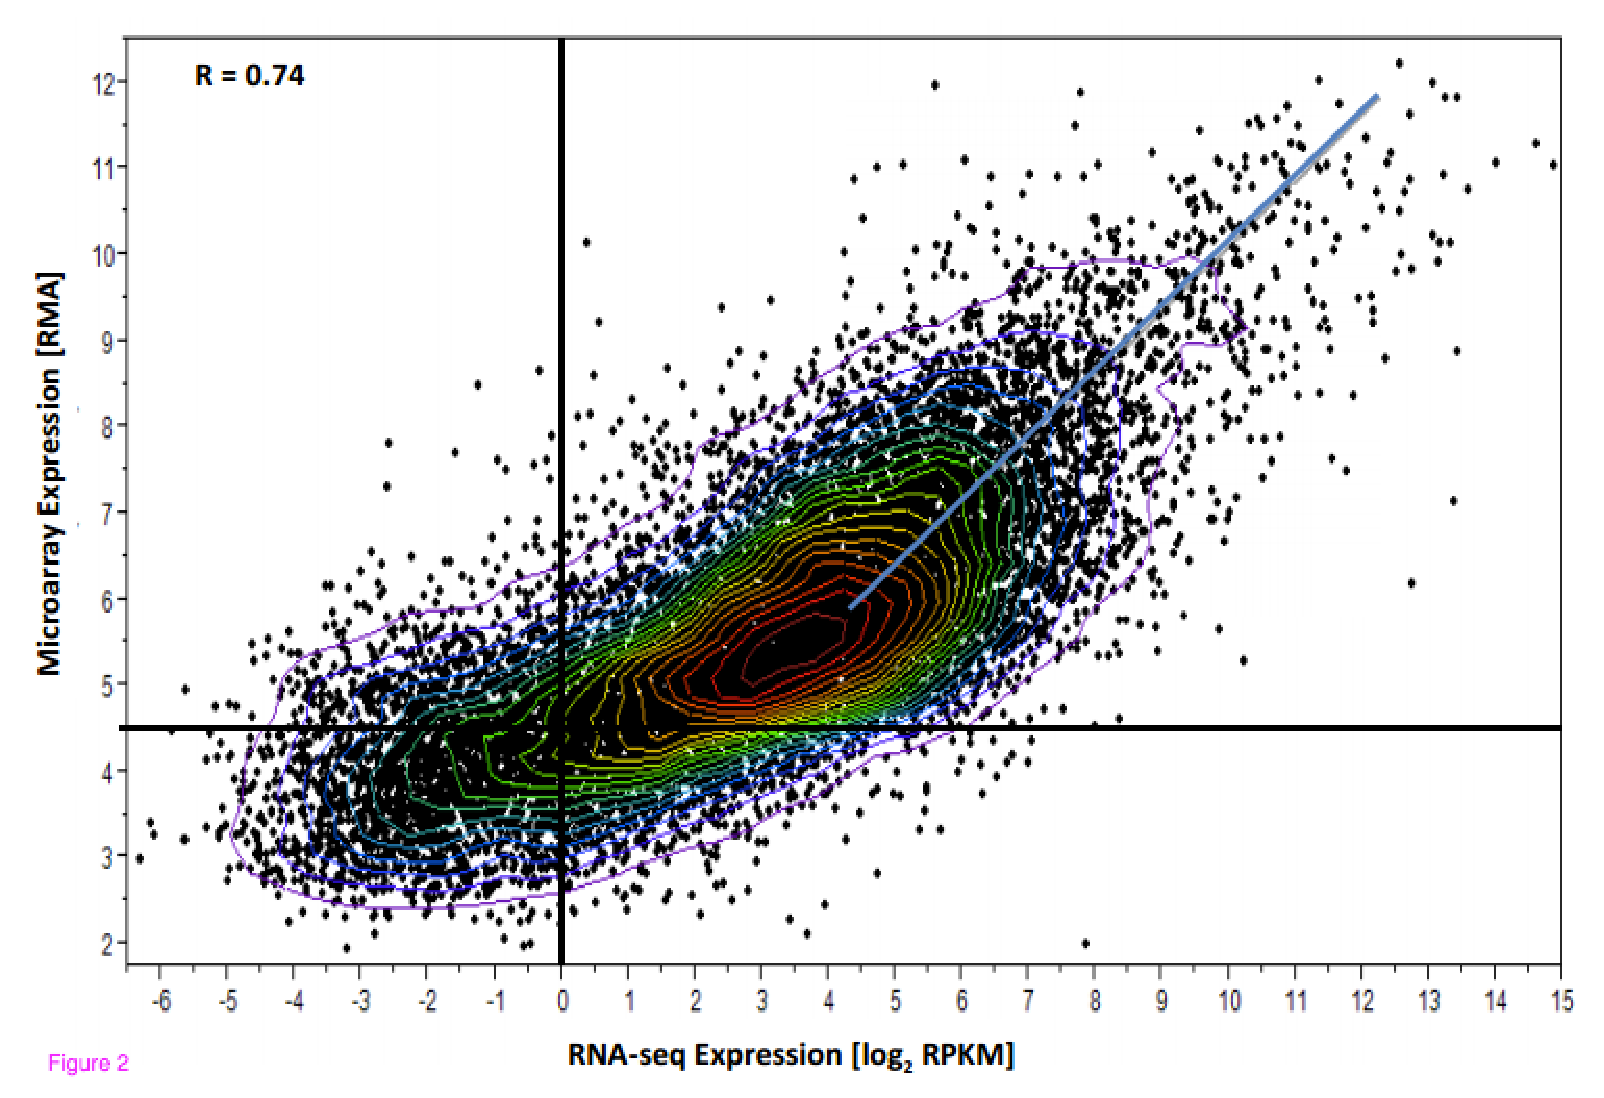
\includegraphics[width=7cm,height=6cm]{Images/Fig2.eps}
%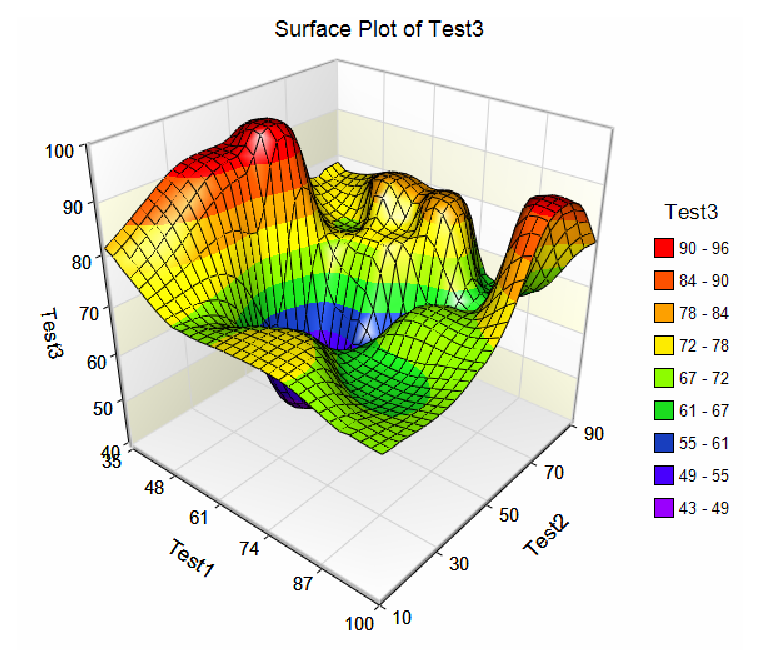
\includegraphics[width=7cm,height=6cm]{Images/Fig1.eps}\\
%\vspace{-0.2cm}
%\caption{\footnotesize{Figure caption should be placed here.}}\label{fig1}
%\end{center}
%\end{figure}
%\section{How to Cite References}
%References must be cited in the text. \cite{Craik:2005}, \cite{Feller:1972}, \cite{Genest:Rivest:1993}, and \cite{LZ15} are some examples of English references.
\section*{Discussion and Conclusion}   
%The conclusion of the article should be presented in a maximum of 3 or 4 lines.
This paper showed that Ranked set sampling significantly improves the estimation of $R=P(X<Y)$ under the Gompertz distribution compared to simple random sampling, especially when distributions are symmetric. The proposed Bayesian estimators are both reliable and economical, making RSS a practical choice for engineering applications with costly measurements.
%\section*{Acknowledgments}   
%If you wish to include acknowledgments, this section should appear before the references.
%%%%%%%%%%%%%%%%%%%%%%%% References %%%%%%%%%%%%%%%%%%%%%%%%%%%%%

\begin{thebibliography}{9}

\bibitem[Aldrabseh et al. (2025)]{aldrabseh2025enhanced}
Aldrabseh M. Z., Ismail M. T., and Al-Omari A. I. (2025), Enhanced estimation of strength-stress reliability using except extreme ranked set sampling under exponential distribution, {\it Life Cycle Reliability and Safety Engineering}, 43(4), 1-19.

\bibitem[Alsadat et al. (2023)]{alsadat2023efficient}
Alsadat N., Hassan A. S., Elgarhy, M., Chesneau C., and Mohamed R. E. (2023), An efficient stress--strength reliability estimate of the unit Gompertz distribution using ranked set sampling, {\it Symmetry}, 15(5), 11-21.

\bibitem[Basikhasteh et al. (2020)]{basikhasteh2020bayesian}
Basikhasteh M., Lak F. and Afshari M. (2020), Bayesian estimation of stress--strength reliability for two-parameter bathtub-shaped lifetime distribution based on maximum ranked set sampling with unequal samples, {\it Journal of Statistical Computation and Simulation}, 90(16), 2975-2990.

\bibitem[Gompertz (1825)]{gompertz1825xxiv}
Gompertz B. (1825), On the nature of the function expressive of the law of human mortality, and on a new mode of determining the value of life contingencies. In a letter to Francis Baily, Esq. FRS \&c, {\it Philosophical transactions of the Royal Society of London,} 115,  513-583.

\bibitem[Hakamipour (2025)]{hakamipour2025stress} 
Hakamipour N. (2025), Stress--strength reliability estimation of s-out-of-k multicomponent systems based on copula function for dependent strength elements under progressively censored sample, {\it International Journal of General Systems,} 54(4), 440-462.

\bibitem[Hudaverdi and  Susam (2023)]{hudaverdi2023copula}
Hudaverdi B. and Susam S. O. (2023), On the copula-based reliability of stress-strength model under bivariate stress, {\it International journal of general systems,} 52(7),  842 - 863.

\bibitem[Karimi Ezmareh and  Yari (2025)]{ezmareh2025exponentiated}
Karimiezmareh Z. and Yari G. (2025), Exponentiated Generalized Exponential Gompertz Distribution: model theory and application, {\it REVSTAT-Statistical Journal}.

\bibitem[Karimi Ezmareh and Yari (2022)]{karimi2022statistical}
Karimi Ezmareh Z. and Yari G. (2022), Statistical Inference of Stress-Strength Reliability of Gompertz Distribution under Type II Censoring, {\it Advances in Mathematical Physics,} 1,  2129677.

\bibitem[Li et al. (1952)]{mcintyre1952method}
McIntyre GA. (1952), A method for unbiased selective sampling, using ranked sets, {\it Australian journal of agricultural research}, 3(4), 385-390.

\bibitem[Lv et al. (2024)]{lv2024statistical}
Lv, Q., Hua R., and Gui W. (2024), Statistical inference of Gompertz distribution under general progressive type II censored competing risks sample, {\it Communications in Statistics-Simulation and Computation}, 53(2), 682-701.

\bibitem[Sindhu et al. (2024)]{sindhu2024generalized}
Sindhu T. N., Shafiq A., and Huassian Z. (2024), Generalized exponentiated unit Gompertz distribution for modeling arthritic pain relief times data: classical approach to statistical inference, {\it Journal of Biopharmaceutical Statistics}, 34(3), 323-348.

\end{thebibliography}
 \end{document}
